\documentclass[twoside]{book}

% Packages required by doxygen
\usepackage{fixltx2e}
\usepackage{calc}
\usepackage{doxygen}
\usepackage[export]{adjustbox} % also loads graphicx
\usepackage{graphicx}
\usepackage[utf8]{inputenc}
\usepackage{makeidx}
\usepackage{multicol}
\usepackage{multirow}
\PassOptionsToPackage{warn}{textcomp}
\usepackage{textcomp}
\usepackage[nointegrals]{wasysym}
\usepackage[table]{xcolor}

% Font selection
\usepackage[T1]{fontenc}
\usepackage[scaled=.90]{helvet}
\usepackage{courier}
\usepackage{amssymb}
\usepackage{sectsty}
\renewcommand{\familydefault}{\sfdefault}
\allsectionsfont{%
  \fontseries{bc}\selectfont%
  \color{darkgray}%
}
\renewcommand{\DoxyLabelFont}{%
  \fontseries{bc}\selectfont%
  \color{darkgray}%
}
\newcommand{\+}{\discretionary{\mbox{\scriptsize$\hookleftarrow$}}{}{}}

% Page & text layout
\usepackage{geometry}
\geometry{%
  a4paper,%
  top=2.5cm,%
  bottom=2.5cm,%
  left=2.5cm,%
  right=2.5cm%
}
\tolerance=750
\hfuzz=15pt
\hbadness=750
\setlength{\emergencystretch}{15pt}
\setlength{\parindent}{0cm}
\setlength{\parskip}{3ex plus 2ex minus 2ex}
\makeatletter
\renewcommand{\paragraph}{%
  \@startsection{paragraph}{4}{0ex}{-1.0ex}{1.0ex}{%
    \normalfont\normalsize\bfseries\SS@parafont%
  }%
}
\renewcommand{\subparagraph}{%
  \@startsection{subparagraph}{5}{0ex}{-1.0ex}{1.0ex}{%
    \normalfont\normalsize\bfseries\SS@subparafont%
  }%
}
\makeatother

% Headers & footers
\usepackage{fancyhdr}
\pagestyle{fancyplain}
\fancyhead[LE]{\fancyplain{}{\bfseries\thepage}}
\fancyhead[CE]{\fancyplain{}{}}
\fancyhead[RE]{\fancyplain{}{\bfseries\leftmark}}
\fancyhead[LO]{\fancyplain{}{\bfseries\rightmark}}
\fancyhead[CO]{\fancyplain{}{}}
\fancyhead[RO]{\fancyplain{}{\bfseries\thepage}}
\fancyfoot[LE]{\fancyplain{}{}}
\fancyfoot[CE]{\fancyplain{}{}}
\fancyfoot[RE]{\fancyplain{}{\bfseries\scriptsize Generated by Doxygen }}
\fancyfoot[LO]{\fancyplain{}{\bfseries\scriptsize Generated by Doxygen }}
\fancyfoot[CO]{\fancyplain{}{}}
\fancyfoot[RO]{\fancyplain{}{}}
\renewcommand{\footrulewidth}{0.4pt}
\renewcommand{\chaptermark}[1]{%
  \markboth{#1}{}%
}
\renewcommand{\sectionmark}[1]{%
  \markright{\thesection\ #1}%
}

% Indices & bibliography
\usepackage{natbib}
\usepackage[titles]{tocloft}
\setcounter{tocdepth}{3}
\setcounter{secnumdepth}{5}
\makeindex

% Hyperlinks (required, but should be loaded last)
\usepackage{ifpdf}
\ifpdf
  \usepackage[pdftex,pagebackref=true]{hyperref}
\else
  \usepackage[ps2pdf,pagebackref=true]{hyperref}
\fi
\hypersetup{%
  colorlinks=true,%
  linkcolor=blue,%
  citecolor=blue,%
  unicode%
}

% Custom commands
\newcommand{\clearemptydoublepage}{%
  \newpage{\pagestyle{empty}\cleardoublepage}%
}

\usepackage{caption}
\captionsetup{labelsep=space,justification=centering,font={bf},singlelinecheck=off,skip=4pt,position=top}

%===== C O N T E N T S =====

\begin{document}

% Titlepage & ToC
\hypersetup{pageanchor=false,
             bookmarksnumbered=true,
             pdfencoding=unicode
            }
\pagenumbering{roman}
\begin{titlepage}
\vspace*{7cm}
\begin{center}%
{\Large libroman \\[1ex]\large 1.\+0 }\\
\vspace*{1cm}
{\large Generated by Doxygen 1.8.11}\\
\end{center}
\end{titlepage}
\clearemptydoublepage
\tableofcontents
\clearemptydoublepage
\pagenumbering{arabic}
\hypersetup{pageanchor=true}

%--- Begin generated contents ---
\chapter{libroman -\/ Documentation}
\label{index}\hypertarget{index}{}This project was made as an assignment for the course {\itshape Métodos de Programação 1} (Programming Methods 101), Computing Department, UnB, April 22nd, 2017. It consists in a library to convert Roman numbers to their integer values.

See the \hyperlink{md_README}{R\+E\+A\+D\+ME} for details about how to build, run and test the library and a little explanation about the inner workings of the Roman numbers.

\subsection*{Development }

I used the test-\/driven development (T\+DD) for the coding of this library. The tests were coded (and then the needed code to satisfy them) and developed as in the sucession below\+:


\begin{DoxyEnumerate}
\item \hyperlink{md_doc_testSimple}{test\+Simple}, where I check if basic input strings are correctly handled.
\item \hyperlink{md_doc_testIncreasing}{test\+Increasing}, where I check if the case in which we have only increasing algarisms.
\item \hyperlink{md_doc_testSubtracting}{test\+Subtracting}, where I check the case for subtracting algarisms, i.\+e., IV or XM.
\item \hyperlink{md_doc_testUntil3000}{test\+Until3000}, where I check from a list from 1 to 3000.
\item \hyperlink{md_doc_testBin}{test\+Bin}, where I check the standalone binary for inconsistencies.
\end{DoxyEnumerate}

The final version of the code library can be found in \hyperlink{roman_8c}{src/roman.\+c} and in \hyperlink{roman-to-int_8c}{src/roman-\/to-\/int.\+c} , the final version of the standalone binary.

\subsection*{Test code coverage }

I then checked the test coverage using the gcov tool, yielding the following results\+:


\begin{DoxyCode}
gcov obj/roman.o
File \textcolor{stringliteral}{'src/roman.c'}
Lines executed:100.00% of 64
\end{DoxyCode}



\begin{DoxyCode}
gcov obj/roman-to-\textcolor{keywordtype}{int}.o
File \textcolor{stringliteral}{'src/roman-to-int.c'}
Lines executed:90.48% of 21
\end{DoxyCode}


In the \hyperlink{roman-to-int_8c}{src/roman-\/to-\/int.\+c} file, the non-\/executed lines are referring to the check in case malloc() fails, which is a very unlikely case.


\begin{DoxyCode}
\textcolor{keywordflow}{if}(arg\_str == NULL) \{
    fprintf(stderr, \textcolor{stringliteral}{"Couldn't allocate memory.\(\backslash\)n"});
    \textcolor{keywordflow}{return} 1;
\}
\end{DoxyCode}


The corresponding .gcov files can be found in the following links\+: roman.\+c.\+gcov and roman-\/to-\/int.\+c.\+gcov

\subsection*{Static analysis }

I ran the command {\ttfamily cppcheck -\/-\/enable=warning .} in the source code directory, obtaining the following results\+:


\begin{DoxyCode}
Checking src/roman-to-\textcolor{keywordtype}{int}.c...
1/7 files checked 14% done
Checking src/roman.c...
2/7 files checked 28% done
Checking test/testBin.c...
3/7 files checked 42% done
Checking test/testIncreasing.c...
4/7 files checked 57% done
Checking test/testSimple.c...
5/7 files checked 71% done
Checking test/testSubtracting.c...
6/7 files checked 85% done
Checking test/testUntil3000.c...
7/7 files checked 100% done
\end{DoxyCode}
 
\chapter{libroman}
\label{md_README}
\hypertarget{md_README}{}
A library to convert Roman numerals to their integer values.

\subsection*{Building the library }

To build the static library, you\textquotesingle{}ll need the following commands available in your system\+:


\begin{DoxyItemize}
\item {\ttfamily g++} (C++ compiler)
\item {\ttfamily ar} (static library creator)
\item {\ttfamily pthreads}
\item {\ttfamily cmake}
\end{DoxyItemize}

In addition, to run the tests you need to have the G\+Test framework in your system. The easiest way is to clone the \href{https://github.com/google/googletest}{\tt Google Test repository} to a directory in your local path and then build it using {\ttfamily cmake}\+:


\begin{DoxyCode}
1 cd /home/foo/
2 git clone https://github.com/google/googletest
3 cd googletest
4 mkdir build && cd build
5 cmake .. && make
\end{DoxyCode}


You can then {\ttfamily cd} to this project root folder {\ttfamily libroman} and pass the G\+Test root directory as the variable {\ttfamily G\+T\+E\+S\+T\+\_\+\+R\+O\+O\+T\+\_\+\+D\+IR} to the {\ttfamily make} command. 
\begin{DoxyCode}
1 cd /home/foo/libroman
2 make GTEST\_ROOT\_DIR=/home/foo/googletest
\end{DoxyCode}


If not, you\textquotesingle{}ll need to provide the paths to G\+Test as variables to the {\ttfamily make} command\+:


\begin{DoxyCode}
1 cd /home/foo/libroman
2 make GTEST\_LIB\_DIR=/home/foo/gtest-lib-path GTEST\_INCLUDE\_DIR=/home/foo/gtest-include-path
\end{DoxyCode}



\begin{DoxyItemize}
\item {\ttfamily G\+T\+E\+S\+T\+\_\+\+L\+I\+B\+\_\+\+D\+IR} points to where the library .a file is. Defaults to {\ttfamily G\+T\+E\+S\+T\+\_\+\+R\+O\+O\+T\+\_\+\+D\+I\+R/build/googlemock/gtest}.
\item {\ttfamily G\+T\+E\+S\+T\+\_\+\+I\+N\+C\+L\+U\+D\+E\+\_\+\+D\+IR} must point to where the include directory {\ttfamily gtest} is. {\ttfamily Defaults to G\+T\+E\+S\+T\+\_\+\+R\+O\+O\+T\+\_\+\+D\+I\+R/googletest/include}.
\end{DoxyItemize}

To run the tests, simply run {\ttfamily make run-\/tests}.

\subsection*{Using the library }

To use the library, simply include the header \hyperlink{roman_8h}{roman.\+h} and call the function \hyperlink{roman_8c_a5d15ad3ed29e4dc0fed9b718523c48c8}{roman\+\_\+to\+\_\+int()} with a string as its only parameter\+:


\begin{DoxyCode}
\textcolor{preprocessor}{#include <stdio.h>}
\textcolor{preprocessor}{#include "\hyperlink{roman_8h}{roman.h}"}

\textcolor{keywordtype}{int} \hyperlink{roman-to-int_8c_a0ddf1224851353fc92bfbff6f499fa97}{main}() \{
    \textcolor{keywordtype}{int} value = \hyperlink{roman_8c_a5d15ad3ed29e4dc0fed9b718523c48c8}{roman\_to\_int}(\textcolor{stringliteral}{"XII"});
    printf(\textcolor{stringliteral}{"%d\(\backslash\)n"}, value); \textcolor{comment}{// 12}
\}
\end{DoxyCode}


And then you need to compile your program linking it against the {\ttfamily libroman.\+a} static library in the {\ttfamily lib/} directory, including the header directory as well\+:


\begin{DoxyCode}
1 g++ -o bar bar.c -I /home/foo/libroman/include -L /home/foo/libroman/lib -lroman
\end{DoxyCode}


\subsection*{Using the standalone binary }

There\textquotesingle{}s a standalone binary {\ttfamily roman-\/to-\/int} in the {\ttfamily bin/} directory that accepts Roman numerical strings as its only command-\/line argument, and prints to stdout its numerical integer value. For example, the code below outputs {\ttfamily 12}\+:


\begin{DoxyCode}
1 cd /home/foo/libroman
2 ./bin/roman-to-int XII
\end{DoxyCode}


\subsection*{Documentation }

To read the docs, go to {\ttfamily doc/html/index.\+html} in your browser or open the file {\ttfamily doc/latex/refman.\+pdf}.

\subsection*{Roman numerical system }

The Roman numerical system is composed by assigning numerical values to certain characters, as in the table below\+:

\tabulinesep=1mm
\begin{longtabu} spread 0pt [c]{*2{|X[-1]}|}
\hline
\rowcolor{\tableheadbgcolor}{\bf Character }&{\bf Value  }\\\cline{1-2}
\endfirsthead
\hline
\endfoot
\hline
\rowcolor{\tableheadbgcolor}{\bf Character }&{\bf Value  }\\\cline{1-2}
\endhead
I &1 \\\cline{1-2}
V &5 \\\cline{1-2}
X &10 \\\cline{1-2}
L &50 \\\cline{1-2}
C &100 \\\cline{1-2}
D &500 \\\cline{1-2}
M &1000 \\\cline{1-2}
\end{longtabu}
The numbers must normally be written in descending order, with repeating characters having their value multiplied by the number of times they appear (3, at most). As such, we\textquotesingle{}d have VI = 6, M\+M\+M\+LX = 3060, for instance. The characters V, L and D cannot be repeated in any circunstance, rendering Roman numbers such as VV or M\+D\+DI invalid.

If a character like I, X or C appears before another with a greater value, its value is subtracted from this one\+: IV = 4, for instance. The rules for subtracting characters are written in the table below\+:

\tabulinesep=1mm
\begin{longtabu} spread 0pt [c]{*2{|X[-1]}|}
\hline
\rowcolor{\tableheadbgcolor}{\bf Character }&{\bf Can appear before  }\\\cline{1-2}
\endfirsthead
\hline
\endfoot
\hline
\rowcolor{\tableheadbgcolor}{\bf Character }&{\bf Can appear before  }\\\cline{1-2}
\endhead
I &V, X \\\cline{1-2}
X &L, C \\\cline{1-2}
C &D, M \\\cline{1-2}
V, L, D &None \\\cline{1-2}
\end{longtabu}
When subtracting there can\textquotesingle{}t be any repetition, thus I\+IX or C\+C\+MI are invalid Roman numbers. 
\chapter{Simple tests}
\label{md_doc_testSimple}
\hypertarget{md_doc_testSimple}{}
Starting with tests for simple inputs\+: \hyperlink{test_simple_8c}{test/test\+Simple.\+c}

\subsection*{First test -\/ sanity of the input }

The first test I did just checks if the function handles correctly non-\/valid strings i.\+e., empty or N\+U\+LL strings\+:


\begin{DoxyCodeInclude}
\hyperlink{test_simple_8c_aff9fa977573ddab7597e233f1775d7c5}{TEST}(SimpleInput, InvalidInput) \{
    EXPECT\_EQ(\hyperlink{roman_8c_a5d15ad3ed29e4dc0fed9b718523c48c8}{roman\_to\_int}(NULL), -1);
    EXPECT\_EQ(\hyperlink{roman_8c_a5d15ad3ed29e4dc0fed9b718523c48c8}{roman\_to\_int}(\textcolor{stringliteral}{""}), -1);
\}
\end{DoxyCodeInclude}


\subsection*{Second test -\/ single characters }

The second test involves checking if the conversion for single characters is working as expected\+:


\begin{DoxyCodeInclude}
\hyperlink{test_simple_8c_aff9fa977573ddab7597e233f1775d7c5}{TEST}(SimpleInput, SingleCharacter) \{
    EXPECT\_EQ(\hyperlink{roman_8c_a5d15ad3ed29e4dc0fed9b718523c48c8}{roman\_to\_int}(\textcolor{stringliteral}{"I"}), 1);
    EXPECT\_EQ(\hyperlink{roman_8c_a5d15ad3ed29e4dc0fed9b718523c48c8}{roman\_to\_int}(\textcolor{stringliteral}{"V"}), 5);
    EXPECT\_EQ(\hyperlink{roman_8c_a5d15ad3ed29e4dc0fed9b718523c48c8}{roman\_to\_int}(\textcolor{stringliteral}{"X"}), 10);
    EXPECT\_EQ(\hyperlink{roman_8c_a5d15ad3ed29e4dc0fed9b718523c48c8}{roman\_to\_int}(\textcolor{stringliteral}{"L"}), 50);
    EXPECT\_EQ(\hyperlink{roman_8c_a5d15ad3ed29e4dc0fed9b718523c48c8}{roman\_to\_int}(\textcolor{stringliteral}{"C"}), 100);
    EXPECT\_EQ(\hyperlink{roman_8c_a5d15ad3ed29e4dc0fed9b718523c48c8}{roman\_to\_int}(\textcolor{stringliteral}{"D"}), 500);
    EXPECT\_EQ(\hyperlink{roman_8c_a5d15ad3ed29e4dc0fed9b718523c48c8}{roman\_to\_int}(\textcolor{stringliteral}{"M"}), 1000);
\}
\end{DoxyCodeInclude}
 The resulting code after these tests can be seen in this \href{https://github.com/diogenes1oliveira/libroman/commit/e9c1c6680af03fe397e5194c65434c857d4dd20d?diff=split#diff-3d6fc1bf772186c45fcd2c22d7ecd7b4}{\tt Git\+Hub commit}. In a nutshell, I added a test for the validity of the string, making the function {\ttfamily \hyperlink{roman_8c_a5d15ad3ed29e4dc0fed9b718523c48c8}{roman\+\_\+to\+\_\+int()}} pass the first test. Then I added the function {\ttfamily single\+\_\+character\+\_\+value()} to return the numerical value of a Roman character, satisfying the second test. 
\chapter{Increasing characters}
\label{md_doc_testIncreasing}
\hypertarget{md_doc_testIncreasing}{}
Tests for more complex inputs\+: \hyperlink{test_increasing_8c}{test/test\+Increasing.\+c}

\subsection*{First test -\/ multiple single characters }

The first test I did checks if the function is returning the right values for strings with repeatable characters (I, X, C and M).


\begin{DoxyCodeInclude}
\hyperlink{test_simple_8c_aff9fa977573ddab7597e233f1775d7c5}{TEST}(ComplexInput, MultipleSingleCharacters) \{
    EXPECT\_EQ(\hyperlink{roman_8c_a5d15ad3ed29e4dc0fed9b718523c48c8}{roman\_to\_int}(\textcolor{stringliteral}{"II"}), 2);
    EXPECT\_EQ(\hyperlink{roman_8c_a5d15ad3ed29e4dc0fed9b718523c48c8}{roman\_to\_int}(\textcolor{stringliteral}{"XXX"}), 30);
    EXPECT\_EQ(\hyperlink{roman_8c_a5d15ad3ed29e4dc0fed9b718523c48c8}{roman\_to\_int}(\textcolor{stringliteral}{"L"}), 50);
    EXPECT\_EQ(\hyperlink{roman_8c_a5d15ad3ed29e4dc0fed9b718523c48c8}{roman\_to\_int}(\textcolor{stringliteral}{"CC"}), 200);
    EXPECT\_EQ(\hyperlink{roman_8c_a5d15ad3ed29e4dc0fed9b718523c48c8}{roman\_to\_int}(\textcolor{stringliteral}{"CCC"}), 300);
    EXPECT\_EQ(\hyperlink{roman_8c_a5d15ad3ed29e4dc0fed9b718523c48c8}{roman\_to\_int}(\textcolor{stringliteral}{"MM"}), 2000);
\}
\end{DoxyCodeInclude}
 This test was satisfied by creating a loop through the string to add all the values in it, as can be seen in this \href{https://github.com/diogenes1oliveira/libroman/commit/637a23468d94b2257037522e7fdd3f34160322ab#diff-3d6fc1bf772186c45fcd2c22d7ecd7b4}{\tt Git\+Hub commit}.

\subsection*{Second test -\/ increasing characters }

The first test I did just checks if the function handles correctly inputs with multiple, but strictly increasing values for its algarisms.


\begin{DoxyCodeInclude}
\hyperlink{test_simple_8c_aff9fa977573ddab7597e233f1775d7c5}{TEST}(ComplexInput, IncreasingCharacters) \{
    EXPECT\_EQ(\hyperlink{roman_8c_a5d15ad3ed29e4dc0fed9b718523c48c8}{roman\_to\_int}(\textcolor{stringliteral}{"XI"}), 11);
    EXPECT\_EQ(\hyperlink{roman_8c_a5d15ad3ed29e4dc0fed9b718523c48c8}{roman\_to\_int}(\textcolor{stringliteral}{"XII"}), 12);
    EXPECT\_EQ(\hyperlink{roman_8c_a5d15ad3ed29e4dc0fed9b718523c48c8}{roman\_to\_int}(\textcolor{stringliteral}{"VI"}), 6);
    EXPECT\_EQ(\hyperlink{roman_8c_a5d15ad3ed29e4dc0fed9b718523c48c8}{roman\_to\_int}(\textcolor{stringliteral}{"LX"}), 60);
    EXPECT\_EQ(\hyperlink{roman_8c_a5d15ad3ed29e4dc0fed9b718523c48c8}{roman\_to\_int}(\textcolor{stringliteral}{"MDXX"}), 1520);
\}
\end{DoxyCodeInclude}
 \subsection*{Third test -\/ non-\/repeatable characters }

This snippet checks if the function fails (as expected) for strings where one of the non-\/repeatable characters (V, L or D) appear more than once.


\begin{DoxyCodeInclude}
\hyperlink{test_simple_8c_aff9fa977573ddab7597e233f1775d7c5}{TEST}(ComplexInput, NonRepeatableCharacters) \{
    EXPECT\_EQ(\hyperlink{roman_8c_a5d15ad3ed29e4dc0fed9b718523c48c8}{roman\_to\_int}(\textcolor{stringliteral}{"VV"}), -1);
    EXPECT\_EQ(\hyperlink{roman_8c_a5d15ad3ed29e4dc0fed9b718523c48c8}{roman\_to\_int}(\textcolor{stringliteral}{"DDD"}), -1);
    EXPECT\_EQ(\hyperlink{roman_8c_a5d15ad3ed29e4dc0fed9b718523c48c8}{roman\_to\_int}(\textcolor{stringliteral}{"LL"}), -1);
    EXPECT\_EQ(\hyperlink{roman_8c_a5d15ad3ed29e4dc0fed9b718523c48c8}{roman\_to\_int}(\textcolor{stringliteral}{"MDDX"}), -1);
\}
\end{DoxyCodeInclude}
 \subsection*{Fourth test -\/ too many repetitions }

This snippet checks if the function fails when the repeatable characters (I, X, C or D) repeat more than 3 times.


\begin{DoxyCodeInclude}
\hyperlink{test_simple_8c_aff9fa977573ddab7597e233f1775d7c5}{TEST}(ComplexInput, TooManyRepetitions) \{
    EXPECT\_EQ(\hyperlink{roman_8c_a5d15ad3ed29e4dc0fed9b718523c48c8}{roman\_to\_int}(\textcolor{stringliteral}{"XXXXX"}), -1);
    EXPECT\_EQ(\hyperlink{roman_8c_a5d15ad3ed29e4dc0fed9b718523c48c8}{roman\_to\_int}(\textcolor{stringliteral}{"MMMM"}), -1);
    EXPECT\_EQ(\hyperlink{roman_8c_a5d15ad3ed29e4dc0fed9b718523c48c8}{roman\_to\_int}(\textcolor{stringliteral}{"IIIIIIII"}), -1);
    
    EXPECT\_EQ(\hyperlink{roman_8c_a5d15ad3ed29e4dc0fed9b718523c48c8}{roman\_to\_int}(\textcolor{stringliteral}{"MIIII"}), -1);
    EXPECT\_EQ(\hyperlink{roman_8c_a5d15ad3ed29e4dc0fed9b718523c48c8}{roman\_to\_int}(\textcolor{stringliteral}{"DXXXX"}), -1);
    EXPECT\_EQ(\hyperlink{roman_8c_a5d15ad3ed29e4dc0fed9b718523c48c8}{roman\_to\_int}(\textcolor{stringliteral}{"LXXXXX"}), -1);
    EXPECT\_EQ(\hyperlink{roman_8c_a5d15ad3ed29e4dc0fed9b718523c48c8}{roman\_to\_int}(\textcolor{stringliteral}{"MMMMMDXII"}), -1);
\}
\end{DoxyCodeInclude}
 To satisfy the 2nd, 3rd and 4th tests, the function was altered as in this \href{https://github.com/diogenes1oliveira/libroman/commit/2da558c048fbe2a989ed9bceddb52fc4b1b615b7#diff-3d6fc1bf772186c45fcd2c22d7ecd7b4}{\tt Github commit}. I added a check function to see if the character is repeatable and then, in the main {\ttfamily \hyperlink{roman_8c_a5d15ad3ed29e4dc0fed9b718523c48c8}{roman\+\_\+to\+\_\+int()}} function, I checked if the repeatable ones weren\textquotesingle{}t repeating too much (more than 3 times).

\subsection*{Fifth test -\/ invalid characters }

This test checks if the function behaves correctly when a string with invalid characters is passed as the input\+:


\begin{DoxyCodeInclude}
\hyperlink{test_simple_8c_aff9fa977573ddab7597e233f1775d7c5}{TEST}(ComplexInput, InvalidCharacter) \{
    EXPECT\_EQ(\hyperlink{roman_8c_a5d15ad3ed29e4dc0fed9b718523c48c8}{roman\_to\_int}(\textcolor{stringliteral}{"A"}), -1);
    EXPECT\_EQ(\hyperlink{roman_8c_a5d15ad3ed29e4dc0fed9b718523c48c8}{roman\_to\_int}(\textcolor{stringliteral}{"XXe"}), -1);
    EXPECT\_EQ(\hyperlink{roman_8c_a5d15ad3ed29e4dc0fed9b718523c48c8}{roman\_to\_int}(\textcolor{stringliteral}{"xx"}), -1);
    EXPECT\_EQ(\hyperlink{roman_8c_a5d15ad3ed29e4dc0fed9b718523c48c8}{roman\_to\_int}(\textcolor{stringliteral}{"AMMMI"}), -1);
    EXPECT\_EQ(\hyperlink{roman_8c_a5d15ad3ed29e4dc0fed9b718523c48c8}{roman\_to\_int}(\textcolor{stringliteral}{"C "}), -1);
    EXPECT\_EQ(\hyperlink{roman_8c_a5d15ad3ed29e4dc0fed9b718523c48c8}{roman\_to\_int}(\textcolor{stringliteral}{"D  I"}), -1);
    EXPECT\_EQ(\hyperlink{roman_8c_a5d15ad3ed29e4dc0fed9b718523c48c8}{roman\_to\_int}(\textcolor{stringliteral}{"MM\_1"}), -1);
\}
\end{DoxyCodeInclude}
 In this \href{https://github.com/diogenes1oliveira/libroman/commit/818abdde2a85e1c1924458c4f25cfff65835bc95#diff-3d6fc1bf772186c45fcd2c22d7ecd7b4}{\tt Github commit}, I made the function comply to this test by making it return {\ttfamily -\/1} when encountering an invalid character. 
\chapter{Subtracting}
\label{md_doc_testSubtracting}
\hypertarget{md_doc_testSubtracting}{}
Tests for subtracting characters\+: \hyperlink{test_subtracting_8c}{test/test\+Subtracting.\+c}

\subsection*{First test -\/ wrong order }

This test checks if the function is failing for subtracting characters in the wrong order, i.\+e.\+: V, L or D before a higher value algarism.


\begin{DoxyCodeInclude}
\hyperlink{test_simple_8c_aff9fa977573ddab7597e233f1775d7c5}{TEST}(SubtractingInput, WrongOrder) \{
    EXPECT\_EQ(\hyperlink{roman_8c_a5d15ad3ed29e4dc0fed9b718523c48c8}{roman\_to\_int}(\textcolor{stringliteral}{"ICCV"}), -1);
    EXPECT\_EQ(\hyperlink{roman_8c_a5d15ad3ed29e4dc0fed9b718523c48c8}{roman\_to\_int}(\textcolor{stringliteral}{"IM"}), -1);
    EXPECT\_EQ(\hyperlink{roman_8c_a5d15ad3ed29e4dc0fed9b718523c48c8}{roman\_to\_int}(\textcolor{stringliteral}{"IDX"}), -1);
    
    EXPECT\_EQ(\hyperlink{roman_8c_a5d15ad3ed29e4dc0fed9b718523c48c8}{roman\_to\_int}(\textcolor{stringliteral}{"XVX"}), -1);
    EXPECT\_EQ(\hyperlink{roman_8c_a5d15ad3ed29e4dc0fed9b718523c48c8}{roman\_to\_int}(\textcolor{stringliteral}{"DM"}), -1);
    
    EXPECT\_EQ(\hyperlink{roman_8c_a5d15ad3ed29e4dc0fed9b718523c48c8}{roman\_to\_int}(\textcolor{stringliteral}{"LM"}), -1);
    EXPECT\_EQ(\hyperlink{roman_8c_a5d15ad3ed29e4dc0fed9b718523c48c8}{roman\_to\_int}(\textcolor{stringliteral}{"LCIX"}), -1);
\}
\end{DoxyCodeInclude}
 \subsection*{Second test -\/ negative characters }

This one confirms if the function is working correctly for characters with negative value, i.\+e.\+: I appearing V or X, C appearing before D or M, etc.


\begin{DoxyCodeInclude}
\hyperlink{test_simple_8c_aff9fa977573ddab7597e233f1775d7c5}{TEST}(SubtractingInput, SingleSubtractingChar) \{
    EXPECT\_EQ(\hyperlink{roman_8c_a5d15ad3ed29e4dc0fed9b718523c48c8}{roman\_to\_int}(\textcolor{stringliteral}{"IV"}), 4);
    EXPECT\_EQ(\hyperlink{roman_8c_a5d15ad3ed29e4dc0fed9b718523c48c8}{roman\_to\_int}(\textcolor{stringliteral}{"IX"}), 9);
    EXPECT\_EQ(\hyperlink{roman_8c_a5d15ad3ed29e4dc0fed9b718523c48c8}{roman\_to\_int}(\textcolor{stringliteral}{"XCII"}), 92);
    EXPECT\_EQ(\hyperlink{roman_8c_a5d15ad3ed29e4dc0fed9b718523c48c8}{roman\_to\_int}(\textcolor{stringliteral}{"CMLXX"}), 970);
\}
\end{DoxyCodeInclude}
 Both tests were satisfied when I created a helper function to check if the algarism can come before another. \href{https://github.com/diogenes1oliveira/libroman/commit/4311b18560b1ccf7ad2c0f3b5fa90c4d505dd7c0#diff-3d6fc1bf772186c45fcd2c22d7ecd7b4}{\tt Git\+Hub commit}

\subsection*{Third test -\/ multiple negative characters }

This snippet checks if the function fails (as expected) for strings where a negative-\/valued algarism appears more than once.


\begin{DoxyCodeInclude}
\hyperlink{test_simple_8c_aff9fa977573ddab7597e233f1775d7c5}{TEST}(SubtractingInput, MultipleSubtractingChar) \{
    EXPECT\_EQ(\hyperlink{roman_8c_a5d15ad3ed29e4dc0fed9b718523c48c8}{roman\_to\_int}(\textcolor{stringliteral}{"IIX"}), -1);
    EXPECT\_EQ(\hyperlink{roman_8c_a5d15ad3ed29e4dc0fed9b718523c48c8}{roman\_to\_int}(\textcolor{stringliteral}{"IIIV"}), -1);
    EXPECT\_EQ(\hyperlink{roman_8c_a5d15ad3ed29e4dc0fed9b718523c48c8}{roman\_to\_int}(\textcolor{stringliteral}{"XXCVI"}), -1);
    EXPECT\_EQ(\hyperlink{roman_8c_a5d15ad3ed29e4dc0fed9b718523c48c8}{roman\_to\_int}(\textcolor{stringliteral}{"XXCIV"}), -1);
\}
\end{DoxyCodeInclude}
 I made the function satisfy this test by checking if there are repetitions when the function is already in the subtracting mode\+: \href{https://github.com/diogenes1oliveira/libroman/commit/0d80a8dac9f89ff4a4953b23d7aa7936137b7092#diff-3d6fc1bf772186c45fcd2c22d7ecd7b4}{\tt Git\+Hub commit} 
\chapter{Until 3000}
\label{md_doc_testUntil3000}
\hypertarget{md_doc_testUntil3000}{}
Tests for a list until 3000\+: \hyperlink{test_until3000_8c}{test/test\+Until3000.\+c}

\subsection*{First test -\/ until 3000 }

This test reads a table with the Roman numerals from 1 to 3000, to see if the function is working for all these values\+: \href{https://github.com/diogenes1oliveira/libroman/commit/f2da07134c34bde40ee4b86f744e9799e9fe8684#diff-15b74e5de5c5d34117039a1dcc826f5d}{\tt Git\+Hub commit}


\begin{DoxyCodeInclude}
\hyperlink{test_simple_8c_aff9fa977573ddab7597e233f1775d7c5}{TEST}(TestingList, TestingUntil3000) \{
    FILE *fp = fopen(\textcolor{stringliteral}{"test/data/romans-until-3000.dat"}, \textcolor{stringliteral}{"r"});
    ASSERT\_TRUE(fp != NULL);
    \textcolor{keywordtype}{char} buffer[\hyperlink{test_until3000_8c_afff9b137f11d394618b464995fe76f99}{LINE\_MAX\_SIZE}];
    
    \textcolor{keywordflow}{while}(fgets(buffer, \hyperlink{test_until3000_8c_afff9b137f11d394618b464995fe76f99}{LINE\_MAX\_SIZE}, fp)) \{
        \textcolor{keywordtype}{int} value;
        \textcolor{keywordtype}{char} roman[\hyperlink{test_until3000_8c_afff9b137f11d394618b464995fe76f99}{LINE\_MAX\_SIZE}];
        
        \textcolor{keywordflow}{if}(sscanf(buffer, \textcolor{stringliteral}{"%d %49s "}, &value, roman) != 2)
            \textcolor{keywordflow}{continue};
        
        EXPECT\_EQ(\hyperlink{roman_8c_a5d15ad3ed29e4dc0fed9b718523c48c8}{roman\_to\_int}(roman), value);
    \}
    
    fclose(fp);
\}
\end{DoxyCodeInclude}

\chapter{Standalone binary}
\label{md_doc_testBin}
\hypertarget{md_doc_testBin}{}
Simple tests for the standalone binary

\subsection*{First test -\/ standalone binary }

This test just checks if the standalone binary fails when it\textquotesingle{}s passed the wrong command-\/line arguments. \href{https://github.com/diogenes1oliveira/libroman/commit/2430213c9b1377f093efbf6c92b445bf09657653#diff-b71fb74c402a09fc46ed4e34ffe34e75}{\tt Git\+Hub commit}


\begin{DoxyCodeInclude}
\hyperlink{test_simple_8c_aff9fa977573ddab7597e233f1775d7c5}{TEST}(TestingBin, ExitsGracefully) \{
    EXPECT\_NE(system(\textcolor{stringliteral}{"./bin/roman-to-int"}), 0);
    EXPECT\_NE(system(\textcolor{stringliteral}{"./bin/roman-to-int VI 38 --system"}), 0);
    
    EXPECT\_EQ(system(\textcolor{stringliteral}{"./bin/roman-to-int VI"}), 0);
    EXPECT\_EQ(system(\textcolor{stringliteral}{"./bin/roman-to-int mIiI"}), 0);
    
    EXPECT\_NE(system(\textcolor{stringliteral}{"./bin/roman-to-int IM"}), 0);
    EXPECT\_NE(system(\textcolor{stringliteral}{"./bin/roman-to-int XDI"}), 0);
\}
\end{DoxyCodeInclude}

\chapter{File Index}
\section{File List}
Here is a list of all files with brief descriptions\+:\begin{DoxyCompactList}
\item\contentsline{section}{include/\hyperlink{roman_8h}{roman.\+h} }{\pageref{roman_8h}}{}
\item\contentsline{section}{src/\hyperlink{roman-to-int_8c}{roman-\/to-\/int.\+c} }{\pageref{roman-to-int_8c}}{}
\item\contentsline{section}{src/\hyperlink{roman_8c}{roman.\+c} }{\pageref{roman_8c}}{}
\item\contentsline{section}{test/\hyperlink{test_bin_8c}{test\+Bin.\+c} }{\pageref{test_bin_8c}}{}
\item\contentsline{section}{test/\hyperlink{test_increasing_8c}{test\+Increasing.\+c} }{\pageref{test_increasing_8c}}{}
\item\contentsline{section}{test/\hyperlink{test_simple_8c}{test\+Simple.\+c} }{\pageref{test_simple_8c}}{}
\item\contentsline{section}{test/\hyperlink{test_subtracting_8c}{test\+Subtracting.\+c} }{\pageref{test_subtracting_8c}}{}
\item\contentsline{section}{test/\hyperlink{test_until3000_8c}{test\+Until3000.\+c} }{\pageref{test_until3000_8c}}{}
\end{DoxyCompactList}

\chapter{File Documentation}
\hypertarget{test_bin_8md}{}\section{doc/test\+Bin.md File Reference}
\label{test_bin_8md}\index{doc/test\+Bin.\+md@{doc/test\+Bin.\+md}}

\hypertarget{test_increasing_8md}{}\section{docs/test\+Increasing.md File Reference}
\label{test_increasing_8md}\index{docs/test\+Increasing.\+md@{docs/test\+Increasing.\+md}}

\hypertarget{test_simple_8md}{}\section{docs/test\+Simple.md File Reference}
\label{test_simple_8md}\index{docs/test\+Simple.\+md@{docs/test\+Simple.\+md}}

\hypertarget{test_subtracting_8md}{}\section{doc/test\+Subtracting.md File Reference}
\label{test_subtracting_8md}\index{doc/test\+Subtracting.\+md@{doc/test\+Subtracting.\+md}}

\hypertarget{test_until3000_8md}{}\section{doc/test\+Until3000.md File Reference}
\label{test_until3000_8md}\index{doc/test\+Until3000.\+md@{doc/test\+Until3000.\+md}}

\hypertarget{roman_8h}{}\section{include/roman.h File Reference}
\label{roman_8h}\index{include/roman.\+h@{include/roman.\+h}}
This graph shows which files directly or indirectly include this file\+:\nopagebreak
\begin{figure}[H]
\begin{center}
\leavevmode
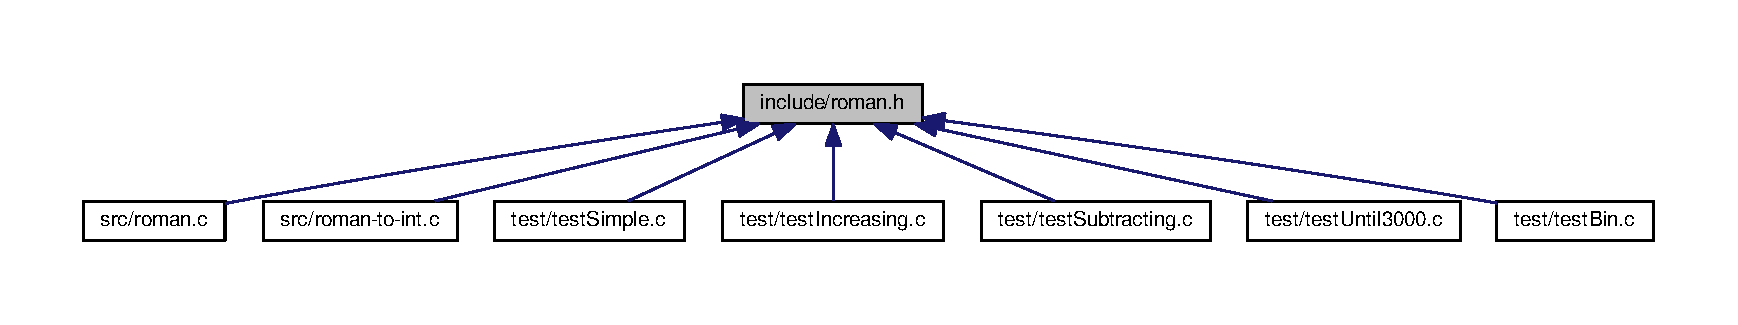
\includegraphics[width=350pt]{roman_8h__dep__incl}
\end{center}
\end{figure}
\subsection*{Functions}
\begin{DoxyCompactItemize}
\item 
int \hyperlink{roman_8h_a5d15ad3ed29e4dc0fed9b718523c48c8}{roman\+\_\+to\+\_\+int} (const char $\ast$input)
\begin{DoxyCompactList}\small\item\em Returns the integer value of the roman characters string. \end{DoxyCompactList}\end{DoxyCompactItemize}


\subsection{Function Documentation}
\index{roman.\+h@{roman.\+h}!roman\+\_\+to\+\_\+int@{roman\+\_\+to\+\_\+int}}
\index{roman\+\_\+to\+\_\+int@{roman\+\_\+to\+\_\+int}!roman.\+h@{roman.\+h}}
\subsubsection[{\texorpdfstring{roman\+\_\+to\+\_\+int(const char $\ast$input)}{roman_to_int(const char *input)}}]{\setlength{\rightskip}{0pt plus 5cm}int roman\+\_\+to\+\_\+int (
\begin{DoxyParamCaption}
\item[{const char $\ast$}]{input}
\end{DoxyParamCaption}
)}\hypertarget{roman_8h_a5d15ad3ed29e4dc0fed9b718523c48c8}{}\label{roman_8h_a5d15ad3ed29e4dc0fed9b718523c48c8}


Returns the integer value of the roman characters string. 

This function parses the input string, which must correspond to a valid roman character string, which must satisfy the following conditions\+:


\begin{DoxyItemize}
\item It must be non-\/null and non-\/empty.
\item The characters V, L or D cannot be repeated.
\item The characters I, X, C or M can be repeated up to three times.
\item If the characters are in non-\/decreasing order 
\end{DoxyItemize}

Definition at line 101 of file roman.\+c.


\hypertarget{mainpage_8dox}{}\section{mainpage.\+dox File Reference}
\label{mainpage_8dox}\index{mainpage.\+dox@{mainpage.\+dox}}

\hypertarget{_r_e_a_d_m_e_8md}{}\section{R\+E\+A\+D\+M\+E.\+md File Reference}
\label{_r_e_a_d_m_e_8md}\index{R\+E\+A\+D\+M\+E.\+md@{R\+E\+A\+D\+M\+E.\+md}}

\hypertarget{roman-to-int_8c}{}\section{src/roman-\/to-\/int.c File Reference}
\label{roman-to-int_8c}\index{src/roman-\/to-\/int.\+c@{src/roman-\/to-\/int.\+c}}
{\ttfamily \#include $<$stdio.\+h$>$}\\*
{\ttfamily \#include $<$stdlib.\+h$>$}\\*
{\ttfamily \#include $<$string.\+h$>$}\\*
{\ttfamily \#include $<$ctype.\+h$>$}\\*
{\ttfamily \#include \char`\"{}roman.\+h\char`\"{}}\\*
Include dependency graph for roman-\/to-\/int.c\+:\nopagebreak
\begin{figure}[H]
\begin{center}
\leavevmode
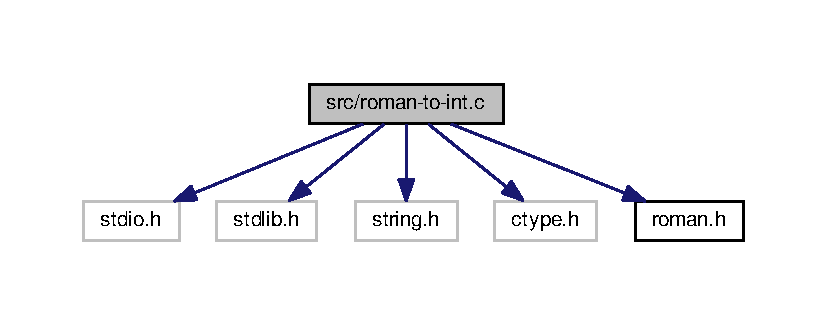
\includegraphics[width=350pt]{roman-to-int_8c__incl}
\end{center}
\end{figure}
\subsection*{Functions}
\begin{DoxyCompactItemize}
\item 
int \hyperlink{roman-to-int_8c_a0ddf1224851353fc92bfbff6f499fa97}{main} (int argc, char $\ast$argv\mbox{[}$\,$\mbox{]})
\end{DoxyCompactItemize}


\subsection{Function Documentation}
\index{roman-\/to-\/int.\+c@{roman-\/to-\/int.\+c}!main@{main}}
\index{main@{main}!roman-\/to-\/int.\+c@{roman-\/to-\/int.\+c}}
\subsubsection[{\texorpdfstring{main(int argc, char $\ast$argv[])}{main(int argc, char *argv[])}}]{\setlength{\rightskip}{0pt plus 5cm}int main (
\begin{DoxyParamCaption}
\item[{int}]{argc, }
\item[{char $\ast$}]{argv\mbox{[}$\,$\mbox{]}}
\end{DoxyParamCaption}
)}\hypertarget{roman-to-int_8c_a0ddf1224851353fc92bfbff6f499fa97}{}\label{roman-to-int_8c_a0ddf1224851353fc92bfbff6f499fa97}


Definition at line 8 of file roman-\/to-\/int.\+c.


\hypertarget{roman_8c}{}\section{src/roman.c File Reference}
\label{roman_8c}\index{src/roman.\+c@{src/roman.\+c}}
{\ttfamily \#include \char`\"{}roman.\+h\char`\"{}}\\*
{\ttfamily \#include $<$stdbool.\+h$>$}\\*
{\ttfamily \#include $<$string.\+h$>$}\\*
Include dependency graph for roman.\+c\+:\nopagebreak
\begin{figure}[H]
\begin{center}
\leavevmode
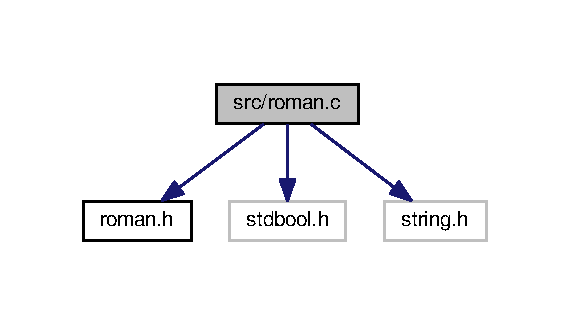
\includegraphics[width=274pt]{roman_8c__incl}
\end{center}
\end{figure}
\subsection*{Functions}
\begin{DoxyCompactItemize}
\item 
static int \hyperlink{roman_8c_a5f42a20564ee7bb82242bc572ad34533}{string\+\_\+length} (const char $\ast$str)
\begin{DoxyCompactList}\small\item\em Returns the length of a valid string. \end{DoxyCompactList}\item 
static int \hyperlink{roman_8c_ab8b51e6124eb6e0c237d64256bde1606}{alg\+\_\+value} (char alg)
\begin{DoxyCompactList}\small\item\em Returns the integer value of a single Roman algarism. \end{DoxyCompactList}\item 
static bool \hyperlink{roman_8c_a4699cffee35f01be5409c50749293337}{alg\+\_\+can\+\_\+repeat} (char alg)
\begin{DoxyCompactList}\small\item\em Checks if the Roman algarism is repeatable (i.\+e., it\textquotesingle{}s not \textquotesingle{}V\textquotesingle{}, \textquotesingle{}L\textquotesingle{} or \textquotesingle{}D\textquotesingle{}). \end{DoxyCompactList}\item 
static bool \hyperlink{roman_8c_afbee2dc5627d75ae539ec36e9fb1a4c6}{alg\+\_\+can\+\_\+come\+\_\+before} (char now, char before)
\begin{DoxyCompactList}\small\item\em Checks if the Roman algarism {\ttfamily now} can come before the character {\ttfamily before} in a valid string, meaning its value is negative. \end{DoxyCompactList}\item 
int \hyperlink{roman_8c_a5d15ad3ed29e4dc0fed9b718523c48c8}{roman\+\_\+to\+\_\+int} (const char $\ast$input)
\begin{DoxyCompactList}\small\item\em Returns the integer value of the roman characters string. \end{DoxyCompactList}\end{DoxyCompactItemize}


\subsection{Function Documentation}
\index{roman.\+c@{roman.\+c}!alg\+\_\+can\+\_\+come\+\_\+before@{alg\+\_\+can\+\_\+come\+\_\+before}}
\index{alg\+\_\+can\+\_\+come\+\_\+before@{alg\+\_\+can\+\_\+come\+\_\+before}!roman.\+c@{roman.\+c}}
\subsubsection[{\texorpdfstring{alg\+\_\+can\+\_\+come\+\_\+before(char now, char before)}{alg_can_come_before(char now, char before)}}]{\setlength{\rightskip}{0pt plus 5cm}static bool alg\+\_\+can\+\_\+come\+\_\+before (
\begin{DoxyParamCaption}
\item[{char}]{now, }
\item[{char}]{before}
\end{DoxyParamCaption}
)\hspace{0.3cm}{\ttfamily [static]}}\hypertarget{roman_8c_afbee2dc5627d75ae539ec36e9fb1a4c6}{}\label{roman_8c_afbee2dc5627d75ae539ec36e9fb1a4c6}


Checks if the Roman algarism {\ttfamily now} can come before the character {\ttfamily before} in a valid string, meaning its value is negative. 

The rules for such preceding characters are as below\+:

\tabulinesep=1mm
\begin{longtabu} spread 0pt [c]{*2{|X[-1]}|}
\hline
\rowcolor{\tableheadbgcolor}{\bf Character }&{\bf Can appear before  }\\\cline{1-2}
\endfirsthead
\hline
\endfoot
\hline
\rowcolor{\tableheadbgcolor}{\bf Character }&{\bf Can appear before  }\\\cline{1-2}
\endhead
\textquotesingle{}I\textquotesingle{} &V, X \\\cline{1-2}
\textquotesingle{}X\textquotesingle{} &L, C \\\cline{1-2}
\textquotesingle{}C\textquotesingle{} &D, M \\\cline{1-2}
\textquotesingle{}V\textquotesingle{}, \textquotesingle{}L\textquotesingle{}, \textquotesingle{}D\textquotesingle{} &None \\\cline{1-2}
\end{longtabu}


Definition at line 85 of file roman.\+c.

\index{roman.\+c@{roman.\+c}!alg\+\_\+can\+\_\+repeat@{alg\+\_\+can\+\_\+repeat}}
\index{alg\+\_\+can\+\_\+repeat@{alg\+\_\+can\+\_\+repeat}!roman.\+c@{roman.\+c}}
\subsubsection[{\texorpdfstring{alg\+\_\+can\+\_\+repeat(char alg)}{alg_can_repeat(char alg)}}]{\setlength{\rightskip}{0pt plus 5cm}static bool alg\+\_\+can\+\_\+repeat (
\begin{DoxyParamCaption}
\item[{char}]{alg}
\end{DoxyParamCaption}
)\hspace{0.3cm}{\ttfamily [static]}}\hypertarget{roman_8c_a4699cffee35f01be5409c50749293337}{}\label{roman_8c_a4699cffee35f01be5409c50749293337}


Checks if the Roman algarism is repeatable (i.\+e., it\textquotesingle{}s not \textquotesingle{}V\textquotesingle{}, \textquotesingle{}L\textquotesingle{} or \textquotesingle{}D\textquotesingle{}). 



Definition at line 69 of file roman.\+c.

\index{roman.\+c@{roman.\+c}!alg\+\_\+value@{alg\+\_\+value}}
\index{alg\+\_\+value@{alg\+\_\+value}!roman.\+c@{roman.\+c}}
\subsubsection[{\texorpdfstring{alg\+\_\+value(char alg)}{alg_value(char alg)}}]{\setlength{\rightskip}{0pt plus 5cm}static int alg\+\_\+value (
\begin{DoxyParamCaption}
\item[{char}]{alg}
\end{DoxyParamCaption}
)\hspace{0.3cm}{\ttfamily [static]}}\hypertarget{roman_8c_ab8b51e6124eb6e0c237d64256bde1606}{}\label{roman_8c_ab8b51e6124eb6e0c237d64256bde1606}


Returns the integer value of a single Roman algarism. 

The corresponding value is given in the table below\+: \tabulinesep=1mm
\begin{longtabu} spread 0pt [c]{*2{|X[-1]}|}
\hline
\rowcolor{\tableheadbgcolor}{\bf Character }&{\bf Value  }\\\cline{1-2}
\endfirsthead
\hline
\endfoot
\hline
\rowcolor{\tableheadbgcolor}{\bf Character }&{\bf Value  }\\\cline{1-2}
\endhead
I &1 \\\cline{1-2}
V &5 \\\cline{1-2}
X &10 \\\cline{1-2}
L &50 \\\cline{1-2}
C &100 \\\cline{1-2}
D &500 \\\cline{1-2}
M &1000 \\\cline{1-2}
\end{longtabu}


Definition at line 34 of file roman.\+c.

\index{roman.\+c@{roman.\+c}!roman\+\_\+to\+\_\+int@{roman\+\_\+to\+\_\+int}}
\index{roman\+\_\+to\+\_\+int@{roman\+\_\+to\+\_\+int}!roman.\+c@{roman.\+c}}
\subsubsection[{\texorpdfstring{roman\+\_\+to\+\_\+int(const char $\ast$input)}{roman_to_int(const char *input)}}]{\setlength{\rightskip}{0pt plus 5cm}int roman\+\_\+to\+\_\+int (
\begin{DoxyParamCaption}
\item[{const char $\ast$}]{input}
\end{DoxyParamCaption}
)}\hypertarget{roman_8c_a5d15ad3ed29e4dc0fed9b718523c48c8}{}\label{roman_8c_a5d15ad3ed29e4dc0fed9b718523c48c8}


Returns the integer value of the roman characters string. 

This function parses the input string, which must correspond to a valid roman character string, which must satisfy the following conditions\+:


\begin{DoxyItemize}
\item It must be non-\/null and non-\/empty.
\item The characters V, L or D cannot be repeated.
\item The characters I, X, C or M can be repeated up to three times.
\item If the characters are in non-\/decreasing order 
\end{DoxyItemize}

Definition at line 101 of file roman.\+c.

\index{roman.\+c@{roman.\+c}!string\+\_\+length@{string\+\_\+length}}
\index{string\+\_\+length@{string\+\_\+length}!roman.\+c@{roman.\+c}}
\subsubsection[{\texorpdfstring{string\+\_\+length(const char $\ast$str)}{string_length(const char *str)}}]{\setlength{\rightskip}{0pt plus 5cm}static int string\+\_\+length (
\begin{DoxyParamCaption}
\item[{const char $\ast$}]{str}
\end{DoxyParamCaption}
)\hspace{0.3cm}{\ttfamily [static]}}\hypertarget{roman_8c_a5f42a20564ee7bb82242bc572ad34533}{}\label{roman_8c_a5f42a20564ee7bb82242bc572ad34533}


Returns the length of a valid string. 

If the string is not valid (i.\+e., N\+U\+LL or empty), returns -\/1. 

Definition at line 12 of file roman.\+c.


\hypertarget{test_bin_8c}{}\section{test/test\+Bin.c File Reference}
\label{test_bin_8c}\index{test/test\+Bin.\+c@{test/test\+Bin.\+c}}
{\ttfamily \#include $<$stdio.\+h$>$}\\*
{\ttfamily \#include $<$stdlib.\+h$>$}\\*
{\ttfamily \#include \char`\"{}gtest/gtest.\+h\char`\"{}}\\*
{\ttfamily \#include \char`\"{}roman.\+h\char`\"{}}\\*
Include dependency graph for test\+Bin.\+c\+:\nopagebreak
\begin{figure}[H]
\begin{center}
\leavevmode
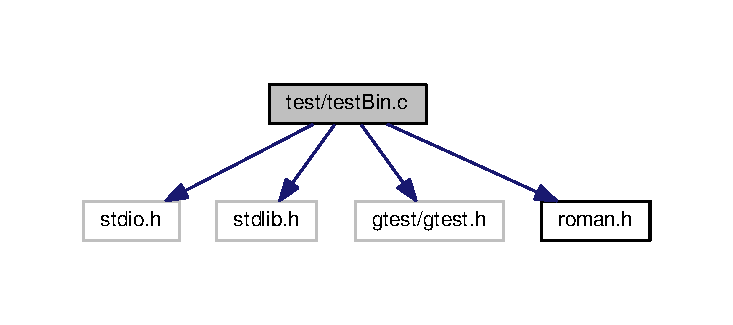
\includegraphics[width=350pt]{test_bin_8c__incl}
\end{center}
\end{figure}
\subsection*{Functions}
\begin{DoxyCompactItemize}
\item 
\hyperlink{test_bin_8c_a85feadc23ad01a2a391deaa1d4d23a76}{T\+E\+ST} (Testing\+Bin, Exits\+Gracefully)
\begin{DoxyCompactList}\small\item\em \mbox{[}Testing\+Bin, Exits\+Gracefully\mbox{]} \end{DoxyCompactList}\item 
int \hyperlink{test_bin_8c_a3c04138a5bfe5d72780bb7e82a18e627}{main} (int argc, char $\ast$$\ast$argv)
\begin{DoxyCompactList}\small\item\em \mbox{[}Testing\+Bin, Exits\+Gracefully\mbox{]} \end{DoxyCompactList}\end{DoxyCompactItemize}


\subsection{Function Documentation}
\index{test\+Bin.\+c@{test\+Bin.\+c}!main@{main}}
\index{main@{main}!test\+Bin.\+c@{test\+Bin.\+c}}
\subsubsection[{\texorpdfstring{main(int argc, char $\ast$$\ast$argv)}{main(int argc, char **argv)}}]{\setlength{\rightskip}{0pt plus 5cm}int main (
\begin{DoxyParamCaption}
\item[{int}]{argc, }
\item[{char $\ast$$\ast$}]{argv}
\end{DoxyParamCaption}
)}\hypertarget{test_bin_8c_a3c04138a5bfe5d72780bb7e82a18e627}{}\label{test_bin_8c_a3c04138a5bfe5d72780bb7e82a18e627}


\mbox{[}Testing\+Bin, Exits\+Gracefully\mbox{]} 



Definition at line 20 of file test\+Bin.\+c.

\index{test\+Bin.\+c@{test\+Bin.\+c}!T\+E\+ST@{T\+E\+ST}}
\index{T\+E\+ST@{T\+E\+ST}!test\+Bin.\+c@{test\+Bin.\+c}}
\subsubsection[{\texorpdfstring{T\+E\+S\+T(\+Testing\+Bin, Exits\+Gracefully)}{TEST(TestingBin, ExitsGracefully)}}]{\setlength{\rightskip}{0pt plus 5cm}T\+E\+ST (
\begin{DoxyParamCaption}
\item[{Testing\+Bin}]{, }
\item[{Exits\+Gracefully}]{}
\end{DoxyParamCaption}
)}\hypertarget{test_bin_8c_a85feadc23ad01a2a391deaa1d4d23a76}{}\label{test_bin_8c_a85feadc23ad01a2a391deaa1d4d23a76}


\mbox{[}Testing\+Bin, Exits\+Gracefully\mbox{]} 



Definition at line 8 of file test\+Bin.\+c.


\hypertarget{test_increasing_8c}{}\section{test/test\+Increasing.c File Reference}
\label{test_increasing_8c}\index{test/test\+Increasing.\+c@{test/test\+Increasing.\+c}}
{\ttfamily \#include \char`\"{}gtest/gtest.\+h\char`\"{}}\\*
{\ttfamily \#include \char`\"{}roman.\+h\char`\"{}}\\*
Include dependency graph for test\+Increasing.\+c\+:\nopagebreak
\begin{figure}[H]
\begin{center}
\leavevmode
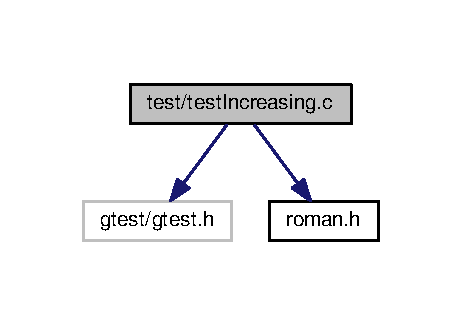
\includegraphics[width=222pt]{test_increasing_8c__incl}
\end{center}
\end{figure}
\subsection*{Functions}
\begin{DoxyCompactItemize}
\item 
\hyperlink{test_increasing_8c_a578c6adf00f73e5f2d177f78b1cc308e}{T\+E\+ST} (Complex\+Input, Increasing\+Characters)
\begin{DoxyCompactList}\small\item\em \mbox{[}Complex\+Input, Increasing\+Characters\mbox{]} \end{DoxyCompactList}\item 
\hyperlink{test_increasing_8c_ae6c8ad374723e2fd0b26e4c8993c60c6}{T\+E\+ST} (Complex\+Input, Invalid\+Character)
\begin{DoxyCompactList}\small\item\em \mbox{[}Complex\+Input, Increasing\+Characters\mbox{]} \end{DoxyCompactList}\item 
\hyperlink{test_increasing_8c_a72add5b20757e98140ffa078f271897b}{T\+E\+ST} (Complex\+Input, Multiple\+Single\+Characters)
\begin{DoxyCompactList}\small\item\em \mbox{[}Complex\+Input, Invalid\+Character\mbox{]} \end{DoxyCompactList}\item 
\hyperlink{test_increasing_8c_a5b30da3eefffcd098caa52400f2fc209}{T\+E\+ST} (Complex\+Input, Non\+Repeatable\+Characters)
\begin{DoxyCompactList}\small\item\em \mbox{[}Complex\+Input, Multiple\+Single\+Characters\mbox{]} \end{DoxyCompactList}\item 
\hyperlink{test_increasing_8c_a1652abfeae14a287b82d1510b9766d53}{T\+E\+ST} (Complex\+Input, Too\+Many\+Repetitions)
\begin{DoxyCompactList}\small\item\em \mbox{[}Complex\+Input, Non\+Repeatable\+Characters\mbox{]} \end{DoxyCompactList}\item 
\hyperlink{test_increasing_8c_a0e7fee3a9d51270a0e9593ef4c14575c}{T\+E\+ST} (Complex\+Input, Subtracting\+Before\+Repetition)
\begin{DoxyCompactList}\small\item\em \mbox{[}Complex\+Input, Too\+Many\+Repetitions\mbox{]} \end{DoxyCompactList}\item 
int \hyperlink{test_increasing_8c_a3c04138a5bfe5d72780bb7e82a18e627}{main} (int argc, char $\ast$$\ast$argv)
\begin{DoxyCompactList}\small\item\em \mbox{[}Complex\+Input, Subtracting\+Before\+Repetition\mbox{]} \end{DoxyCompactList}\end{DoxyCompactItemize}


\subsection{Function Documentation}
\index{test\+Increasing.\+c@{test\+Increasing.\+c}!main@{main}}
\index{main@{main}!test\+Increasing.\+c@{test\+Increasing.\+c}}
\subsubsection[{\texorpdfstring{main(int argc, char $\ast$$\ast$argv)}{main(int argc, char **argv)}}]{\setlength{\rightskip}{0pt plus 5cm}int main (
\begin{DoxyParamCaption}
\item[{int}]{argc, }
\item[{char $\ast$$\ast$}]{argv}
\end{DoxyParamCaption}
)}\hypertarget{test_increasing_8c_a3c04138a5bfe5d72780bb7e82a18e627}{}\label{test_increasing_8c_a3c04138a5bfe5d72780bb7e82a18e627}


\mbox{[}Complex\+Input, Subtracting\+Before\+Repetition\mbox{]} 



Definition at line 67 of file test\+Increasing.\+c.

\index{test\+Increasing.\+c@{test\+Increasing.\+c}!T\+E\+ST@{T\+E\+ST}}
\index{T\+E\+ST@{T\+E\+ST}!test\+Increasing.\+c@{test\+Increasing.\+c}}
\subsubsection[{\texorpdfstring{T\+E\+S\+T(\+Complex\+Input, Increasing\+Characters)}{TEST(ComplexInput, IncreasingCharacters)}}]{\setlength{\rightskip}{0pt plus 5cm}T\+E\+ST (
\begin{DoxyParamCaption}
\item[{Complex\+Input}]{, }
\item[{Increasing\+Characters}]{}
\end{DoxyParamCaption}
)}\hypertarget{test_increasing_8c_a578c6adf00f73e5f2d177f78b1cc308e}{}\label{test_increasing_8c_a578c6adf00f73e5f2d177f78b1cc308e}


\mbox{[}Complex\+Input, Increasing\+Characters\mbox{]} 



Definition at line 5 of file test\+Increasing.\+c.

\index{test\+Increasing.\+c@{test\+Increasing.\+c}!T\+E\+ST@{T\+E\+ST}}
\index{T\+E\+ST@{T\+E\+ST}!test\+Increasing.\+c@{test\+Increasing.\+c}}
\subsubsection[{\texorpdfstring{T\+E\+S\+T(\+Complex\+Input, Invalid\+Character)}{TEST(ComplexInput, InvalidCharacter)}}]{\setlength{\rightskip}{0pt plus 5cm}T\+E\+ST (
\begin{DoxyParamCaption}
\item[{Complex\+Input}]{, }
\item[{Invalid\+Character}]{}
\end{DoxyParamCaption}
)}\hypertarget{test_increasing_8c_ae6c8ad374723e2fd0b26e4c8993c60c6}{}\label{test_increasing_8c_ae6c8ad374723e2fd0b26e4c8993c60c6}


\mbox{[}Complex\+Input, Increasing\+Characters\mbox{]} 

\mbox{[}Complex\+Input, Invalid\+Character\mbox{]} 

Definition at line 15 of file test\+Increasing.\+c.

\index{test\+Increasing.\+c@{test\+Increasing.\+c}!T\+E\+ST@{T\+E\+ST}}
\index{T\+E\+ST@{T\+E\+ST}!test\+Increasing.\+c@{test\+Increasing.\+c}}
\subsubsection[{\texorpdfstring{T\+E\+S\+T(\+Complex\+Input, Multiple\+Single\+Characters)}{TEST(ComplexInput, MultipleSingleCharacters)}}]{\setlength{\rightskip}{0pt plus 5cm}T\+E\+ST (
\begin{DoxyParamCaption}
\item[{Complex\+Input}]{, }
\item[{Multiple\+Single\+Characters}]{}
\end{DoxyParamCaption}
)}\hypertarget{test_increasing_8c_a72add5b20757e98140ffa078f271897b}{}\label{test_increasing_8c_a72add5b20757e98140ffa078f271897b}


\mbox{[}Complex\+Input, Invalid\+Character\mbox{]} 

\mbox{[}Complex\+Input, Multiple\+Single\+Characters\mbox{]} 

Definition at line 27 of file test\+Increasing.\+c.

\index{test\+Increasing.\+c@{test\+Increasing.\+c}!T\+E\+ST@{T\+E\+ST}}
\index{T\+E\+ST@{T\+E\+ST}!test\+Increasing.\+c@{test\+Increasing.\+c}}
\subsubsection[{\texorpdfstring{T\+E\+S\+T(\+Complex\+Input, Non\+Repeatable\+Characters)}{TEST(ComplexInput, NonRepeatableCharacters)}}]{\setlength{\rightskip}{0pt plus 5cm}T\+E\+ST (
\begin{DoxyParamCaption}
\item[{Complex\+Input}]{, }
\item[{Non\+Repeatable\+Characters}]{}
\end{DoxyParamCaption}
)}\hypertarget{test_increasing_8c_a5b30da3eefffcd098caa52400f2fc209}{}\label{test_increasing_8c_a5b30da3eefffcd098caa52400f2fc209}


\mbox{[}Complex\+Input, Multiple\+Single\+Characters\mbox{]} 

\mbox{[}Complex\+Input, Non\+Repeatable\+Characters\mbox{]} 

Definition at line 38 of file test\+Increasing.\+c.

\index{test\+Increasing.\+c@{test\+Increasing.\+c}!T\+E\+ST@{T\+E\+ST}}
\index{T\+E\+ST@{T\+E\+ST}!test\+Increasing.\+c@{test\+Increasing.\+c}}
\subsubsection[{\texorpdfstring{T\+E\+S\+T(\+Complex\+Input, Too\+Many\+Repetitions)}{TEST(ComplexInput, TooManyRepetitions)}}]{\setlength{\rightskip}{0pt plus 5cm}T\+E\+ST (
\begin{DoxyParamCaption}
\item[{Complex\+Input}]{, }
\item[{Too\+Many\+Repetitions}]{}
\end{DoxyParamCaption}
)}\hypertarget{test_increasing_8c_a1652abfeae14a287b82d1510b9766d53}{}\label{test_increasing_8c_a1652abfeae14a287b82d1510b9766d53}


\mbox{[}Complex\+Input, Non\+Repeatable\+Characters\mbox{]} 

\mbox{[}Complex\+Input, Too\+Many\+Repetitions\mbox{]} 

Definition at line 47 of file test\+Increasing.\+c.

\index{test\+Increasing.\+c@{test\+Increasing.\+c}!T\+E\+ST@{T\+E\+ST}}
\index{T\+E\+ST@{T\+E\+ST}!test\+Increasing.\+c@{test\+Increasing.\+c}}
\subsubsection[{\texorpdfstring{T\+E\+S\+T(\+Complex\+Input, Subtracting\+Before\+Repetition)}{TEST(ComplexInput, SubtractingBeforeRepetition)}}]{\setlength{\rightskip}{0pt plus 5cm}T\+E\+ST (
\begin{DoxyParamCaption}
\item[{Complex\+Input}]{, }
\item[{Subtracting\+Before\+Repetition}]{}
\end{DoxyParamCaption}
)}\hypertarget{test_increasing_8c_a0e7fee3a9d51270a0e9593ef4c14575c}{}\label{test_increasing_8c_a0e7fee3a9d51270a0e9593ef4c14575c}


\mbox{[}Complex\+Input, Too\+Many\+Repetitions\mbox{]} 

\mbox{[}Complex\+Input, Subtracting\+Before\+Repetition\mbox{]} 

Definition at line 60 of file test\+Increasing.\+c.


\hypertarget{test_simple_8c}{}\section{test/test\+Simple.c File Reference}
\label{test_simple_8c}\index{test/test\+Simple.\+c@{test/test\+Simple.\+c}}
{\ttfamily \#include \char`\"{}gtest/gtest.\+h\char`\"{}}\\*
{\ttfamily \#include \char`\"{}roman.\+h\char`\"{}}\\*
Include dependency graph for test\+Simple.\+c\+:\nopagebreak
\begin{figure}[H]
\begin{center}
\leavevmode
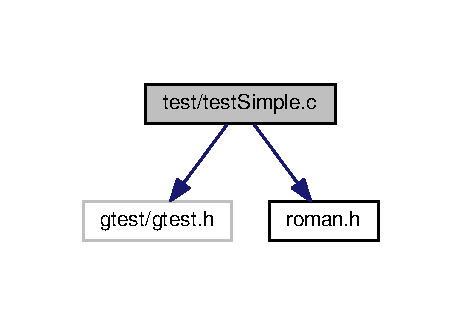
\includegraphics[width=222pt]{test_simple_8c__incl}
\end{center}
\end{figure}
\subsection*{Functions}
\begin{DoxyCompactItemize}
\item 
\hyperlink{test_simple_8c_aff9fa977573ddab7597e233f1775d7c5}{T\+E\+ST} (Simple\+Input, Invalid\+Input)
\begin{DoxyCompactList}\small\item\em \mbox{[}Simple\+Input, Invalid\+Input\mbox{]} \end{DoxyCompactList}\item 
\hyperlink{test_simple_8c_a7780b7f477399a829f64fd94a5423bb6}{T\+E\+ST} (Simple\+Input, Single\+Character)
\begin{DoxyCompactList}\small\item\em \mbox{[}Simple\+Input, Invalid\+Input\mbox{]} \end{DoxyCompactList}\item 
int \hyperlink{test_simple_8c_a3c04138a5bfe5d72780bb7e82a18e627}{main} (int argc, char $\ast$$\ast$argv)
\begin{DoxyCompactList}\small\item\em \mbox{[}Simple\+Input, Single\+Character\mbox{]} \end{DoxyCompactList}\end{DoxyCompactItemize}


\subsection{Function Documentation}
\index{test\+Simple.\+c@{test\+Simple.\+c}!main@{main}}
\index{main@{main}!test\+Simple.\+c@{test\+Simple.\+c}}
\subsubsection[{\texorpdfstring{main(int argc, char $\ast$$\ast$argv)}{main(int argc, char **argv)}}]{\setlength{\rightskip}{0pt plus 5cm}int main (
\begin{DoxyParamCaption}
\item[{int}]{argc, }
\item[{char $\ast$$\ast$}]{argv}
\end{DoxyParamCaption}
)}\hypertarget{test_simple_8c_a3c04138a5bfe5d72780bb7e82a18e627}{}\label{test_simple_8c_a3c04138a5bfe5d72780bb7e82a18e627}


\mbox{[}Simple\+Input, Single\+Character\mbox{]} 



Definition at line 23 of file test\+Simple.\+c.

\index{test\+Simple.\+c@{test\+Simple.\+c}!T\+E\+ST@{T\+E\+ST}}
\index{T\+E\+ST@{T\+E\+ST}!test\+Simple.\+c@{test\+Simple.\+c}}
\subsubsection[{\texorpdfstring{T\+E\+S\+T(\+Simple\+Input, Invalid\+Input)}{TEST(SimpleInput, InvalidInput)}}]{\setlength{\rightskip}{0pt plus 5cm}T\+E\+ST (
\begin{DoxyParamCaption}
\item[{Simple\+Input}]{, }
\item[{Invalid\+Input}]{}
\end{DoxyParamCaption}
)}\hypertarget{test_simple_8c_aff9fa977573ddab7597e233f1775d7c5}{}\label{test_simple_8c_aff9fa977573ddab7597e233f1775d7c5}


\mbox{[}Simple\+Input, Invalid\+Input\mbox{]} 



Definition at line 5 of file test\+Simple.\+c.

\index{test\+Simple.\+c@{test\+Simple.\+c}!T\+E\+ST@{T\+E\+ST}}
\index{T\+E\+ST@{T\+E\+ST}!test\+Simple.\+c@{test\+Simple.\+c}}
\subsubsection[{\texorpdfstring{T\+E\+S\+T(\+Simple\+Input, Single\+Character)}{TEST(SimpleInput, SingleCharacter)}}]{\setlength{\rightskip}{0pt plus 5cm}T\+E\+ST (
\begin{DoxyParamCaption}
\item[{Simple\+Input}]{, }
\item[{Single\+Character}]{}
\end{DoxyParamCaption}
)}\hypertarget{test_simple_8c_a7780b7f477399a829f64fd94a5423bb6}{}\label{test_simple_8c_a7780b7f477399a829f64fd94a5423bb6}


\mbox{[}Simple\+Input, Invalid\+Input\mbox{]} 

\mbox{[}Simple\+Input, Single\+Character\mbox{]} 

Definition at line 12 of file test\+Simple.\+c.


\hypertarget{test_subtracting_8c}{}\section{test/test\+Subtracting.c File Reference}
\label{test_subtracting_8c}\index{test/test\+Subtracting.\+c@{test/test\+Subtracting.\+c}}
{\ttfamily \#include \char`\"{}gtest/gtest.\+h\char`\"{}}\\*
{\ttfamily \#include \char`\"{}roman.\+h\char`\"{}}\\*
Include dependency graph for test\+Subtracting.\+c\+:\nopagebreak
\begin{figure}[H]
\begin{center}
\leavevmode
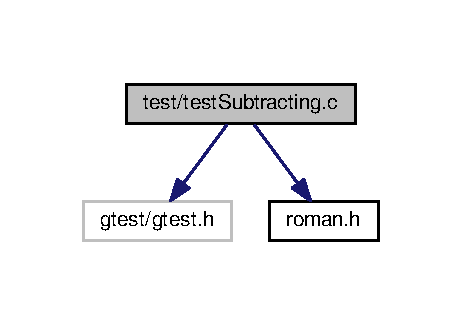
\includegraphics[width=222pt]{test_subtracting_8c__incl}
\end{center}
\end{figure}
\subsection*{Functions}
\begin{DoxyCompactItemize}
\item 
\hyperlink{test_subtracting_8c_a5b85a75cb9b1b65c04b295881185e5fd}{T\+E\+ST} (Subtracting\+Input, Wrong\+Order)
\begin{DoxyCompactList}\small\item\em \mbox{[}Subtracting\+Input, Wrong\+Order\mbox{]} \end{DoxyCompactList}\item 
\hyperlink{test_subtracting_8c_a4a3c4ddd22a00089ba61feb3a72fbbae}{T\+E\+ST} (Subtracting\+Input, Single\+Subtracting\+Char)
\begin{DoxyCompactList}\small\item\em \mbox{[}Subtracting\+Input, Wrong\+Order\mbox{]} \end{DoxyCompactList}\item 
\hyperlink{test_subtracting_8c_a61dc6f312f588f58e5c9d9b5b87c993f}{T\+E\+ST} (Subtracting\+Input, Multiple\+Subtracting\+Char)
\begin{DoxyCompactList}\small\item\em \mbox{[}Subtracting\+Input, Single\+Subtracting\+Char\mbox{]} \end{DoxyCompactList}\item 
int \hyperlink{test_subtracting_8c_a3c04138a5bfe5d72780bb7e82a18e627}{main} (int argc, char $\ast$$\ast$argv)
\begin{DoxyCompactList}\small\item\em \mbox{[}Subtracting\+Input, Multiple\+Subtracting\+Char\mbox{]} \end{DoxyCompactList}\end{DoxyCompactItemize}


\subsection{Function Documentation}
\index{test\+Subtracting.\+c@{test\+Subtracting.\+c}!main@{main}}
\index{main@{main}!test\+Subtracting.\+c@{test\+Subtracting.\+c}}
\subsubsection[{\texorpdfstring{main(int argc, char $\ast$$\ast$argv)}{main(int argc, char **argv)}}]{\setlength{\rightskip}{0pt plus 5cm}int main (
\begin{DoxyParamCaption}
\item[{int}]{argc, }
\item[{char $\ast$$\ast$}]{argv}
\end{DoxyParamCaption}
)}\hypertarget{test_subtracting_8c_a3c04138a5bfe5d72780bb7e82a18e627}{}\label{test_subtracting_8c_a3c04138a5bfe5d72780bb7e82a18e627}


\mbox{[}Subtracting\+Input, Multiple\+Subtracting\+Char\mbox{]} 



Definition at line 36 of file test\+Subtracting.\+c.

\index{test\+Subtracting.\+c@{test\+Subtracting.\+c}!T\+E\+ST@{T\+E\+ST}}
\index{T\+E\+ST@{T\+E\+ST}!test\+Subtracting.\+c@{test\+Subtracting.\+c}}
\subsubsection[{\texorpdfstring{T\+E\+S\+T(\+Subtracting\+Input, Wrong\+Order)}{TEST(SubtractingInput, WrongOrder)}}]{\setlength{\rightskip}{0pt plus 5cm}T\+E\+ST (
\begin{DoxyParamCaption}
\item[{Subtracting\+Input}]{, }
\item[{Wrong\+Order}]{}
\end{DoxyParamCaption}
)}\hypertarget{test_subtracting_8c_a5b85a75cb9b1b65c04b295881185e5fd}{}\label{test_subtracting_8c_a5b85a75cb9b1b65c04b295881185e5fd}


\mbox{[}Subtracting\+Input, Wrong\+Order\mbox{]} 



Definition at line 5 of file test\+Subtracting.\+c.

\index{test\+Subtracting.\+c@{test\+Subtracting.\+c}!T\+E\+ST@{T\+E\+ST}}
\index{T\+E\+ST@{T\+E\+ST}!test\+Subtracting.\+c@{test\+Subtracting.\+c}}
\subsubsection[{\texorpdfstring{T\+E\+S\+T(\+Subtracting\+Input, Single\+Subtracting\+Char)}{TEST(SubtractingInput, SingleSubtractingChar)}}]{\setlength{\rightskip}{0pt plus 5cm}T\+E\+ST (
\begin{DoxyParamCaption}
\item[{Subtracting\+Input}]{, }
\item[{Single\+Subtracting\+Char}]{}
\end{DoxyParamCaption}
)}\hypertarget{test_subtracting_8c_a4a3c4ddd22a00089ba61feb3a72fbbae}{}\label{test_subtracting_8c_a4a3c4ddd22a00089ba61feb3a72fbbae}


\mbox{[}Subtracting\+Input, Wrong\+Order\mbox{]} 

\mbox{[}Subtracting\+Input, Single\+Subtracting\+Char\mbox{]} 

Definition at line 19 of file test\+Subtracting.\+c.

\index{test\+Subtracting.\+c@{test\+Subtracting.\+c}!T\+E\+ST@{T\+E\+ST}}
\index{T\+E\+ST@{T\+E\+ST}!test\+Subtracting.\+c@{test\+Subtracting.\+c}}
\subsubsection[{\texorpdfstring{T\+E\+S\+T(\+Subtracting\+Input, Multiple\+Subtracting\+Char)}{TEST(SubtractingInput, MultipleSubtractingChar)}}]{\setlength{\rightskip}{0pt plus 5cm}T\+E\+ST (
\begin{DoxyParamCaption}
\item[{Subtracting\+Input}]{, }
\item[{Multiple\+Subtracting\+Char}]{}
\end{DoxyParamCaption}
)}\hypertarget{test_subtracting_8c_a61dc6f312f588f58e5c9d9b5b87c993f}{}\label{test_subtracting_8c_a61dc6f312f588f58e5c9d9b5b87c993f}


\mbox{[}Subtracting\+Input, Single\+Subtracting\+Char\mbox{]} 

\mbox{[}Subtracting\+Input, Multiple\+Subtracting\+Char\mbox{]} 

Definition at line 28 of file test\+Subtracting.\+c.


\hypertarget{test_until3000_8c}{}\section{test/test\+Until3000.c File Reference}
\label{test_until3000_8c}\index{test/test\+Until3000.\+c@{test/test\+Until3000.\+c}}
{\ttfamily \#include \char`\"{}gtest/gtest.\+h\char`\"{}}\\*
{\ttfamily \#include \char`\"{}roman.\+h\char`\"{}}\\*
Include dependency graph for test\+Until3000.\+c\+:\nopagebreak
\begin{figure}[H]
\begin{center}
\leavevmode
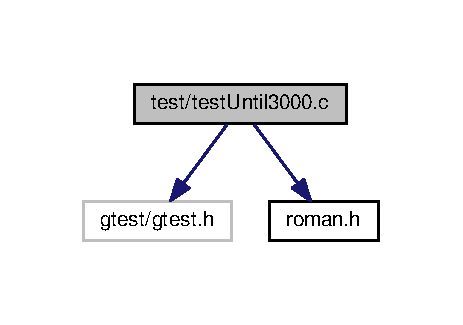
\includegraphics[width=222pt]{test_until3000_8c__incl}
\end{center}
\end{figure}
\subsection*{Macros}
\begin{DoxyCompactItemize}
\item 
\#define \hyperlink{test_until3000_8c_afff9b137f11d394618b464995fe76f99}{L\+I\+N\+E\+\_\+\+M\+A\+X\+\_\+\+S\+I\+ZE}~50
\end{DoxyCompactItemize}
\subsection*{Functions}
\begin{DoxyCompactItemize}
\item 
\hyperlink{test_until3000_8c_ae56c17e7745f0e7d9ad4f166d306e0c3}{T\+E\+ST} (Testing\+List, Testing\+Until3000)
\begin{DoxyCompactList}\small\item\em \mbox{[}Testing\+List, Testing\+Until3000\mbox{]} \end{DoxyCompactList}\item 
int \hyperlink{test_until3000_8c_a3c04138a5bfe5d72780bb7e82a18e627}{main} (int argc, char $\ast$$\ast$argv)
\begin{DoxyCompactList}\small\item\em \mbox{[}Testing\+List, Testing\+Until3000\mbox{]} \end{DoxyCompactList}\end{DoxyCompactItemize}


\subsection{Macro Definition Documentation}
\index{test\+Until3000.\+c@{test\+Until3000.\+c}!L\+I\+N\+E\+\_\+\+M\+A\+X\+\_\+\+S\+I\+ZE@{L\+I\+N\+E\+\_\+\+M\+A\+X\+\_\+\+S\+I\+ZE}}
\index{L\+I\+N\+E\+\_\+\+M\+A\+X\+\_\+\+S\+I\+ZE@{L\+I\+N\+E\+\_\+\+M\+A\+X\+\_\+\+S\+I\+ZE}!test\+Until3000.\+c@{test\+Until3000.\+c}}
\subsubsection[{\texorpdfstring{L\+I\+N\+E\+\_\+\+M\+A\+X\+\_\+\+S\+I\+ZE}{LINE_MAX_SIZE}}]{\setlength{\rightskip}{0pt plus 5cm}\#define L\+I\+N\+E\+\_\+\+M\+A\+X\+\_\+\+S\+I\+ZE~50}\hypertarget{test_until3000_8c_afff9b137f11d394618b464995fe76f99}{}\label{test_until3000_8c_afff9b137f11d394618b464995fe76f99}


Definition at line 4 of file test\+Until3000.\+c.



\subsection{Function Documentation}
\index{test\+Until3000.\+c@{test\+Until3000.\+c}!main@{main}}
\index{main@{main}!test\+Until3000.\+c@{test\+Until3000.\+c}}
\subsubsection[{\texorpdfstring{main(int argc, char $\ast$$\ast$argv)}{main(int argc, char **argv)}}]{\setlength{\rightskip}{0pt plus 5cm}int main (
\begin{DoxyParamCaption}
\item[{int}]{argc, }
\item[{char $\ast$$\ast$}]{argv}
\end{DoxyParamCaption}
)}\hypertarget{test_until3000_8c_a3c04138a5bfe5d72780bb7e82a18e627}{}\label{test_until3000_8c_a3c04138a5bfe5d72780bb7e82a18e627}


\mbox{[}Testing\+List, Testing\+Until3000\mbox{]} 



Definition at line 26 of file test\+Until3000.\+c.

\index{test\+Until3000.\+c@{test\+Until3000.\+c}!T\+E\+ST@{T\+E\+ST}}
\index{T\+E\+ST@{T\+E\+ST}!test\+Until3000.\+c@{test\+Until3000.\+c}}
\subsubsection[{\texorpdfstring{T\+E\+S\+T(\+Testing\+List, Testing\+Until3000)}{TEST(TestingList, TestingUntil3000)}}]{\setlength{\rightskip}{0pt plus 5cm}T\+E\+ST (
\begin{DoxyParamCaption}
\item[{Testing\+List}]{, }
\item[{Testing\+Until3000}]{}
\end{DoxyParamCaption}
)}\hypertarget{test_until3000_8c_ae56c17e7745f0e7d9ad4f166d306e0c3}{}\label{test_until3000_8c_ae56c17e7745f0e7d9ad4f166d306e0c3}


\mbox{[}Testing\+List, Testing\+Until3000\mbox{]} 



Definition at line 7 of file test\+Until3000.\+c.


%--- End generated contents ---

% Index
\backmatter
\newpage
\phantomsection
\clearemptydoublepage
\addcontentsline{toc}{chapter}{Index}
\printindex

\end{document}
